\documentclass{article}
\usepackage{tikz}
\usetikzlibrary{arrows.meta,positioning,calc,shapes.geometric}
\pagestyle{empty}
\begin{document}
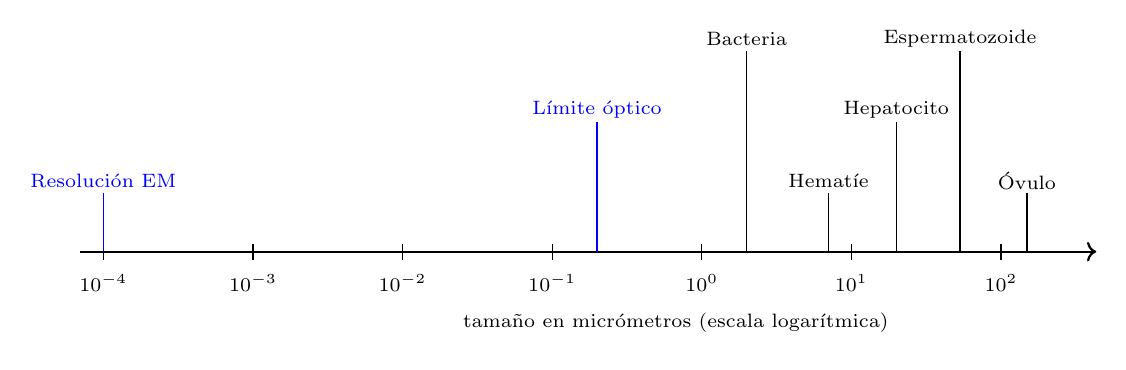
\begin{tikzpicture}
\draw[thick,->] (-0.3,0) -- (12.61,0);
\draw (0.00,0.1) -- (0.00,-0.1); \node[font=\scriptsize] at (0.00,-0.4) {$10^{-4}$};
\draw (1.90,0.1) -- (1.90,-0.1); \node[font=\scriptsize] at (1.90,-0.4) {$10^{-3}$};
\draw (3.80,0.1) -- (3.80,-0.1); \node[font=\scriptsize] at (3.80,-0.4) {$10^{-2}$};
\draw (5.70,0.1) -- (5.70,-0.1); \node[font=\scriptsize] at (5.70,-0.4) {$10^{-1}$};
\draw (7.60,0.1) -- (7.60,-0.1); \node[font=\scriptsize] at (7.60,-0.4) {$10^{0}$};
\draw (9.50,0.1) -- (9.50,-0.1); \node[font=\scriptsize] at (9.50,-0.4) {$10^{1}$};
\draw (11.40,0.1) -- (11.40,-0.1); \node[font=\scriptsize] at (11.40,-0.4) {$10^{2}$};
\draw[blue] (0.00,0) -- (0.00,0.75); \node[blue, font=\scriptsize, fill=white, inner sep=1pt] at (0.00,0.90) {Resolución EM};
\draw[blue] (6.27,0) -- (6.27,1.65); \node[blue, font=\scriptsize, fill=white, inner sep=1pt] at (6.27,1.80) {Límite óptico};
\draw[black] (8.17,0) -- (8.17,2.55); \node[black, font=\scriptsize, fill=white, inner sep=1pt] at (8.17,2.70) {Bacteria};
\draw[black] (9.21,0) -- (9.21,0.75); \node[black, font=\scriptsize, fill=white, inner sep=1pt] at (9.21,0.90) {Hematíe};
\draw[black] (10.07,0) -- (10.07,1.65); \node[black, font=\scriptsize, fill=white, inner sep=1pt] at (10.07,1.80) {Hepatocito};
\draw[black] (10.88,0) -- (10.88,2.55); \node[black, font=\scriptsize, fill=white, inner sep=1pt] at (10.88,2.70) {Espermatozoide};
\draw[black] (11.73,0) -- (11.73,0.75); \node[black, font=\scriptsize, fill=white, inner sep=1pt] at (11.73,0.90) {Óvulo};
\node[font=\scriptsize] at (7.27,-0.9) {tamaño en micrómetros (escala logarítmica)};
\end{tikzpicture}
\end{document}
